\setproblem{30985}

\begin{frame}[label=p2]{직장인 파댕이의 사회생활(30985)}

\tiny

\begin{block}{문제}
파댕이는 중견기업 회사에서 직장인으로 일하고 있다. 사장님이 직장인 파댕이를 무척 아끼기 때문에, 파댕이는 사장실에 찾아가 사장님께 인사를 하려고 한다.

직장인 파댕이의 회사가 있는 건물은 $K$층으로 구성되어 있는데 각 층은 방과 복도로 구성되어 있다. 복도를 통해 방과 방 사이를 양방향으로 이동할 수 있다. 모든 층은 같은 모습을 하고 있다.

파댕이는 현재 $1$층의 $1$번 방에 있고, 사장실은 $K$층의 $N$번 방이다. 파댕이는 현재 자신의 위치에서부터 사장실까지 최소 시간을 사용하여 도착할 방법을 찾아야 한다.

파댕이는 각각의 복도를 지나가는 데 걸리는 시간이 얼마인지 알고 있다. 더불어 어떤 방에는 엘리베이터가 있어서 그 엘리베이터를 타고 위층으로 올라갈 수 있다. 한 층의 $i$번 방에 설치된 엘리베이터는 다른 층에 있는 모든 $i$번 방을 연결한다.

특정 엘리베이터에만 사람이 몰릴 수 있기 때문에 어떤 엘리베이터는 빠르고 어떤 엘리베이터는 느릴 수 있다. 파댕이는 각각의 엘리베이터가 한 층을 올라가는 데 걸리는 시간이 얼마인지도 알고 있다.

건물의 모습과 엘리베이터의 속도가 주어지면, 파댕이가 사장실까지 가는 최소 시간을 계산하는 프로그램을 작성하시오.
\end{block}

\begin{block}{입력}
첫째 줄에 방의 수 $N\ (2 \leq N \leq 100{,}000)$과 복도의 수 $M\ (1 \leq M \leq 300{,}000)$, 건물의 층수 $K\ (2 \leq K \leq 200{,}000)$가 공백으로 구분되어 주어진다.

다음 줄부터 $M$개의 줄에 걸쳐 세 정수 $u, v, c$가 공백으로 구분되어 주어진다. $(1 \leq u, v \leq N, 1 \leq c \leq 100{,}000{,}000, u \neq v)$ 이는 $u$번 방과 $v$번 방을 잇는 복도가 존재하며 이를 지나가는 데 걸리는 시간이 $c$라는 뜻이다.

임의의 서로 다른 두 방에 대해 한쪽 방에서 다른 쪽 방으로 이어진 복도는 $1$개 이하다.

다음 줄에 $N$개의 정수 $e_1, \cdots, e_N$이 공백으로 구분되어 주어진다. $(e_i = -1 \text{ or } 1 \leq e_i \leq 100{,}000{,}000)$ 이는 $i$번째 방에 존재하는 엘리베이터를 타면 한 층을 올라갈 때마다 $e_i$의 시간이 든다는 뜻이다.

만약 $i$번째 방에 엘리베이터가 존재하지 않는다면, $e_i = -1$이다.
\end{block}

\end{frame}

\begin{frame}{예제}
\begin{center}
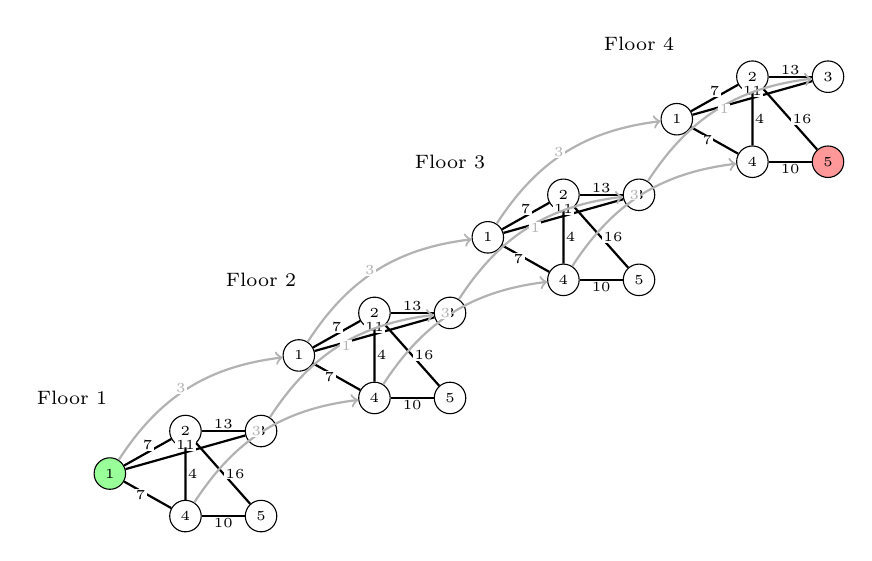
\begin{tikzpicture}[
    scale=0.6,
    vertex/.style={circle, draw, minimum size=4mm, inner sep=0pt, font=\tiny},
    start/.style={circle, draw, fill=green!40, minimum size=4mm, inner sep=0pt, font=\tiny},
    goal/.style={circle, draw, fill=red!40, minimum size=4mm, inner sep=0pt, font=\tiny},
    edge/.style={thick},
    elev/.style={->, thick, gray!60},
    wlabel/.style={font=\tiny, fill=white, inner sep=0.5pt},
]

% ---- base layout ----
\def\xA{0}   \def\yA{0}
\def\xB{1.6} \def\yB{0.9}
\def\xC{3.2} \def\yC{0.9}
\def\xD{1.6} \def\yD{-0.9}
\def\xE{3.2} \def\yE{-0.9}

% ---- floor spacing ----
\def\dx{4}
\def\dy{2.5}

% ---- draw floors ----
\foreach \f in {1,2,3,4} {
  \begin{scope}[shift={({(\f-1)*\dx},{(\f-1)*\dy})}]

    % 시작점 / 끝점 스타일 적용
    \ifnum\f=1
        \node[start] (v1-\f) at (\xA,\yA) {1};
    \else
        \node[vertex] (v1-\f) at (\xA,\yA) {1};
    \fi

    \node[vertex] (v2-\f) at (\xB,\yB) {2};
    \node[vertex] (v3-\f) at (\xC,\yC) {3};
    \node[vertex] (v4-\f) at (\xD,\yD) {4};

    \ifnum\f=4
        \node[goal] (v5-\f) at (\xE,\yE) {5};
    \else
        \node[vertex] (v5-\f) at (\xE,\yE) {5};
    \fi

    \draw[edge] (v1-\f) -- node[wlabel, above] {7} (v2-\f);
    \draw[edge] (v1-\f) -- node[wlabel, above] {11} (v3-\f);
    \draw[edge] (v1-\f) -- node[wlabel, left] {7} (v4-\f);
    \draw[edge] (v2-\f) -- node[wlabel, above] {13} (v3-\f);
    \draw[edge] (v2-\f) -- node[wlabel, right] {4} (v4-\f);
    \draw[edge] (v2-\f) -- node[wlabel, right] {16} (v5-\f);
    \draw[edge] (v4-\f) -- node[wlabel, below] {10} (v5-\f);

    \node[font=\scriptsize] at (-0.8,1.6) {Floor \f};

  \end{scope}
}

% ---- elevators (curved) ----
\foreach \f in {1,2,3} {
  \draw[elev] (v1-\f) to[bend left=25] node[wlabel, left] {3} (v1-\the\numexpr\f+1\relax);
  \draw[elev] (v3-\f) to[bend left=25] node[wlabel, right] {1} (v3-\the\numexpr\f+1\relax);
  \draw[elev] (v4-\f) to[bend left=25] node[wlabel, left] {3} (v4-\the\numexpr\f+1\relax);
}

\end{tikzpicture}
\end{center}
\end{frame}

\begin{frame}{풀이}
\footnotesize

\begin{itemize}
  \item 엘레베이터는 반드시 $1$층에서 타서 $K$층까지 한 번에 간다고 생각하더라도 최적해를 구할 수 있습니다.
  \item 모든 엘리베이터 $e_1, e_2, \cdots, e_N$를 시작점으로 해서 $1$번방과 $N$번방 까지의 경로를 구할 수도 있습니다.
  \item 반대로 $1$번 방과 $N$번 방을 시작점으로 해서 모든 엘리베이터까지의 경로를 구할 수도 있습니다.
\end{itemize}

\end{frame}

\begin{frame}[fragile, allowframebreaks]{원찬혁 소스 코드}
\inputminted{java}{../src/\prob/chanhyeok/Main.java}
\end{frame}

\begin{frame}[fragile, allowframebreaks]{정의찬 소스 코드}
\inputminted{java}{../src/\prob/uichan/Main.java}
\end{frame}

\begin{frame}[fragile, allowframebreaks]{서민종 소스 코드}
\inputminted{java}{../src/\prob/minjong/Main.java}
\end{frame}

\begin{frame}[fragile, allowframebreaks]{김준형 소스 코드}
\inputminted{java}{../src/\prob/junhyeong/Main.java}
\end{frame}

\begin{frame}[fragile, allowframebreaks]{김지훈 소스 코드}
\inputminted{java}{../src/\prob/jihoon/BOJ_30985.java}
\end{frame}

\begin{frame}[fragile, allowframebreaks]{임건애 소스 코드}
\inputminted{java}{../src/\prob/keonae/Main.java}
\end{frame}

\begin{frame}[fragile, allowframebreaks]{김시온 소스 코드}
\inputminted{java}{../src/\prob/sion/Main.java}
\end{frame}
